% This is "sig-alternate.tex" V2.1 April 2013
% This file should be compiled with V2.5 of "sig-alternate.cls" May 2012
%
% This example file demonstrates the use of the 'sig-alternate.cls'
% V2.5 LaTeX2e document class file. It is for those submitting
% articles to ACM Conference Proceedings WHO DO NOT WISH TO
% STRICTLY ADHERE TO THE SIGS (PUBS-BOARD-ENDORSED) STYLE.
% The 'sig-alternate.cls' file will produce a similar-looking,
% albeit, 'tighter' paper resulting in, invariably, fewer pages.
%
% ----------------------------------------------------------------------------------------------------------------
% This .tex file (and associated .cls V2.5) produces:
%       1) The Permission Statement
%       2) The Conference (location) Info information
%       3) The Copyright Line with ACM data
%       4) NO page numbers
%
% as against the acm_proc_article-sp.cls file which
% DOES NOT produce 1) thru' 3) above.
%
% Using 'sig-alternate.cls' you have control, however, from within
% the source .tex file, over both the CopyrightYear
% (defaulted to 200X) and the ACM Copyright Data
% (defaulted to X-XXXXX-XX-X/XX/XX).
% e.g.
% \CopyrightYear{2007} will cause 2007 to appear in the copyright line.
% \crdata{0-12345-67-8/90/12} will cause 0-12345-67-8/90/12 to appear in the copyright line.
%
% ---------------------------------------------------------------------------------------------------------------
% This .tex source is an example which *does* use
% the .bib file (from which the .bbl file % is produced).
% REMEMBER HOWEVER: After having produced the .bbl file,
% and prior to final submission, you *NEED* to 'insert'
% your .bbl file into your source .tex file so as to provide
% ONE 'self-contained' source file.
%
% ================= IF YOU HAVE QUESTIONS =======================
% Questions regarding the SIGS styles, SIGS policies and
% procedures, Conferences etc. should be sent to
% Adrienne Griscti (griscti@acm.org)
%
% Technical questions _only_ to
% Gerald Murray (murray@hq.acm.org)
% ===============================================================
%
% For tracking purposes - this is V2.0 - May 2012




\documentclass{sig-alternate-05-2015}

%\usepackage [english]{babel}
%\usepackage [autostyle, english = american]{csquotes}
%\MakeOuterQuote{"}
\usepackage{lineno}
\begin{document}
\linenumbers
% Copyright
\setcopyright{acmcopyright}
%\setcopyright{acmlicensed}
%\setcopyright{rightsretained}
%\setcopyright{usgov}
%\setcopyright{usgovmixed}
%\setcopyright{cagov}
%\setcopyright{cagovmixed}


% DOI
\doi{10.475/123_4}

% ISBN
\isbn{123-4567-24-567/08/06}

%Conference
\conferenceinfo{PLDI '13}{June 16--19, 2013, Seattle, WA, USA}

\acmPrice{\$15.00}

%
% --- Author Metadata here ---
\conferenceinfo{WOODSTOCK}{'97 El Paso, Texas USA}
%\CopyrightYear{2007} % Allows default copyright year (20XX) to be over-ridden - IF NEED BE.
%\crdata{0-12345-67-8/90/01}  % Allows default copyright data (0-89791-88-6/97/05) to be over-ridden - IF NEED BE.
% --- End of Author Metadata ---

\title{ Mining Pre-Exposure Prophylaxis Trends in Social Media Data}
%
% You need the command \numberofauthors to handle the 'placement
% and alignment' of the authors beneath the title.
%
% For aesthetic reasons, we recommend 'three authors at a time'
% i.e. three 'name/affiliation blocks' be placed beneath the title.
%
% NOTE: You are NOT restricted in how many 'rows' of
% "name/affiliations" may appear. We just ask that you restrict
% the number of 'columns' to three.
%
% Because of the available 'opening page real-estate'
% we ask you to refrain from putting more than six authors
% (two rows with three columns) beneath the article title.
% More than six makes the first-page appear very cluttered indeed.
%
% Use the \alignauthor commands to handle the names
% and affiliations for an 'aesthetic maximum' of six authors.
% Add names, affiliations, addresses for
% the seventh etc. author(s) as the argument for the
% \additionalauthors command.
% These 'additional authors' will be output/set for you
% without further effort on your part as the last section in
% the body of your article BEFORE References or any Appendices.

\numberofauthors{2} %  in this sample file, there are a *total*
% of EIGHT authors. SIX appear on the 'first-page' (for formatting
% reasons) and the remaining two appear in the \additionalauthors section.
%
\author{
% You can go ahead and credit any number of authors here,
% e.g. one 'row of three' or two rows (consisting of one row of three
% and a second row of one, two or three).
%
% The command \alignauthor (no curly braces needed) should
% precede each author name, affiliation/snail-mail address and
% e-mail address. Additionally, tag each line of
% affiliation/address with \affaddr, and tag the
% e-mail address with \email.
%
% 1st. author
\alignauthor
Patrick Breen\\
       \affaddr{Institute of Bioinformatics}\\
       \affaddr{The University of Georgia}\\
       \affaddr{Athens, Georgia}\\
       \email{pbreen@uga.edu}
% 2nd. author
\alignauthor
Shannon Quinn\titlenote{Corresponding author.}\\
       \affaddr{Department of Computer Science}\\
       \affaddr{University of Georgia}\\
       \affaddr{Athens, Georgia}\\
       \email{squinn@cs.uga.edu}
}



\maketitle
\begin{abstract}

Pre-Exposure Prophylaxis (PrEP) is a recently developed therapy for the prevention of Human Immunodeficiency Virus (HIV) transmission. The treatment is available as a pill named Truvada and is taken once a day by HIV negative individuals for as much as 99\% protection when exposed to HIV. While medically effective, PrEP suffers from high drug costs, HIV-related social stigma, and under-informed health providers and patients. Data mining of social media has proven effective in the monitoring of HIV in the United States, but no study has investigated PrEP using social media. This paper describes a data mining and machine learning strategy using natural language processing (NLP), that monitors Twitter social media data to identify PrEP discussion trends. Our results show that we can identify PrEP and HIV discussion dynamics over time, and PrEP-related tweets with positive and negative sentiment. These results can be used by public health professionals to monitor PrEP discussion trends, and identify strategies to improve HIV prevention.

%These methods may also be useful to identify and preempt HIV outbreaks before they reach epidemic levels.

\end{abstract}


%
% The code below should be generated by the tool at
% http://dl.acm.org/ccs.cfm
% Please copy and paste the code instead of the example below. 
%

\begin{CCSXML}
<ccs2012>
<concept>
<concept_id>10010405.10010444.10010449</concept_id>
<concept_desc>Applied computing~Health informatics</concept_desc>
<concept_significance>500</concept_significance>
</concept>
<concept>
<concept_id>10010147.10010257.10010293.10010309.10011671</concept_id>
<concept_desc>Computing methodologies~Latent Dirichlet allocation</concept_desc>
<concept_significance>300</concept_significance>
</concept>
<concept>
<concept_id>10010147.10010257.10010293.10010319</concept_id>
<concept_desc>Computing methodologies~Learning latent representations</concept_desc>
<concept_significance>300</concept_significance>
</concept>
</ccs2012>
\end{CCSXML}

\ccsdesc[500]{Applied computing~Health informatics}
\ccsdesc[300]{Computing methodologies~Latent Dirichlet allocation}
\ccsdesc[300]{Computing methodologies~Learning latent representations}

\ccsdesc[500]{Applied computing~Health informatics}


%
% End generated code
%

%
%  Use this command to print the description
%
\printccsdesc

% We no longer use \terms command
%\terms{Theory}

\keywords{ Social Media, HIV, Topic Modeling, Document Classification}

\section{Introduction}
Pre-exposure prophylaxis (PrEP), a treatment for the prevention of Immunodeficiency Virus (HIV), is marketed under the trade name Truvada. Truvada was approved by the Food and Drug Administration (FDA) in 2012 to prevent sexually acquired HIV infection after several positive trials~\cite{grant2010preexposure,thigpen2012antiretroviral} showed that it was safe and effective. Despite minimal side effects, and risk protection of up to 99\%, PrEP suffers from uncertain health insurance compensation, the risk of producing drug resistant strains, and uninformed health providers and patients~\cite{liu2014early}. Truvada must be taken once a day for full protection. In some individuals, adherence is difficult to maintain~\cite{van2012unraveling}, leading to loss of Truvada's effectiveness. While public health officials can spread information and monitor the effectiveness of PrEP at the clinic-level, scaled-up data mining on social media data may provide more complete information on PrEP at the national level.

Tweets from Twitter consist of short 140 character text messages that may also contain hashtag annotations. Twitter has been used as a source of data for large scale opinion mining in public health monitoring contexts, to predict the spread of influenza~\cite{aramaki2011twitter}, predict postpartum depression~\cite{de2013predicting}, and examine tobacco use~\cite{myslin2013using}. Recently it has also been used for the study of HIV~\cite{young2014methods,young2013online}. These studies of HIV have focused on county-level HIV prevalence prediction, and general HIV discussion monitoring, but they have not focused on PrEP-related discussion. Furthermore, existing HIV social media analyses have not taken full advantage of natural language processing (NLP) techniques to discover semantic information in unstructured text~\cite{young2015big}.

One recently developed tool for NLP, called Word2Vec, is a connectionist method that embeds words as word-vectors in a semantic space that captures substitution-similarity~\cite{mikolov2013efficient}. There are several forms of Word2Vec, though the most popular version, Skip-gram Negative Sampling (SGNS), has been shown to perform well at producing word-vectors that capture important word relationships. This includes most notably word analogies. 

Word2Vec is also used as a preprocessing step for additional analyses that start from pre-trained word-vectors. Doc2Vec~\cite{le2014distributed} is a method that produces a document-vector for each document, and each document-level identifier. In the case of a tweet-corpus, document identifiers might include for example document ID, hashtags, and the user who created the document. Each of these document-level identifiers is embedded in a similarity space, allowing one to identify similar tweets, hastags, and users.

Latent Dirichlet Allocation~\cite{blei2003latent} (LDA) is used to identify a small set of latent topics present in an unstructured corpus. LDA is a graphical model that generates documents from a set of latent topics. A topic is a probability distribution over words that captures a set of related words. LDA models are often inferred in practice using Bayesian inference either via collapsed Gibbs sampling or variational Bayesian methods. Inspection of the resulting topics allows one to identify relevant terms and the context in which they occur in the corpus. 

Dynamic Topic Modeling~\cite{blei2006dynamic} (DTM) is an extension of LDA that produces a series of topic models over time. Briefly, the documents in the corpus are divided into several corpora that are successive in time. LDA is performed on each corpus to extract a topic distribution. The posterior topic distribution from time $t_n$ is used as the prior for time $t_{n+1}$. This lets the DTM model determine a topic model for each time point that is dependent both on the set of tweets from that time point, and on the previous time point's topic distribution.

In this paper we respond to the acknowledged need to harness large scale data in the battle against HIV~\cite{young2015big}. We use the above NLP techniques to extract PrEP-related semantic information from a Twitter corpus dataset. We identify critical PrEP related terms, users, hashtags and tweets. We identify PrEP discussion trends over time, and identify other topics that people who tweet about PrEP, also tweet about. Finally we train a sentiment classifier that automatically identifies PrEP-related tweets with positive and negative sentiment. Together these results, and these approaches, can be used by public health officials to identify trends in the national PrEP discussion and respond to public health issues as they arise.

\section{Results}
We sought to determine trends in HIV and PrEP discourse on twitter to inform and coordinate public health efforts aiming to promote PrEP adoption and adherence for at-risk individuals. We collected 624,569 tweets containing at least one of the following words 'HIV', 'AIDS', 'truvada', 'prophylaxis', 'imtesting', or 'PrEP' from Twitter's streaming API. The tweets were restricted to English language, and the collection dates spanned from the 47th week of 2015 to the 14th week of 2016. The tweets were cleaned of exotic characters. Before performing topic analysis, we excluded words that were mentioned fewer than 10 times, or more than 0.3 times the number of documents. We also performed Term Frequency Inverse Document Frequency (TF-IDF) normalization.

We excluded tweets that did not originate in contiguous United States time zones. A subset of 14,204 tweets (about 2\%) had geolocation coordinates available. We found that these tweets were largely concentrated on US and Canadian metro areas (Figure 1). The tweets did not seem to be over represented in any geographical region of the US.

% figure 1
\begin{figure}
\centering
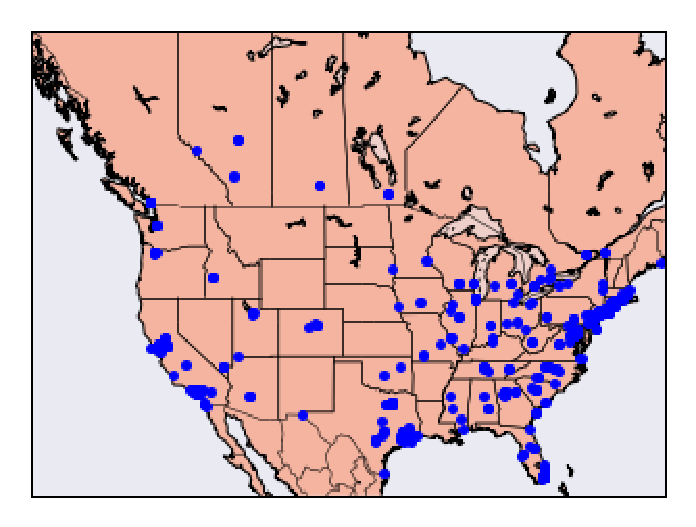
\includegraphics[height=3in, width=4in]{map}
\caption{Plot of geolocated tweets.}
\end{figure}

\subsection{Word and Document Similarity}

The first analysis that we performed sought to identify certain keywords, hashtags, tweets and users, that were discussed in HIV and PrEP related contexts. Word2Vec and the related method, Doc2Vec are unsupervised machine learning methods that have performed well at embedding natural language in a semantic vector space. In our analysis, Word2Vec allows us to determine semantically similar words to a query word, while Doc2Vec allows us to determine similar tweets, users and hashtags to a query hashtag.

We trained a Word2Vec model, and queried for the top 10 word-vectors related to the term PrEP (Table 1). We found several HIV/AIDS related events, WorldAIDSDay, HLM2016AIDS, ICASA2015, as well as the PrEP drug Truvada, and the term HIV. In addition, we found the acronym ART which refers to Anti-Retroviral Therapy. DoingIt, and OneConversation, are ongoing efforts led by the Center for Disease Control (CDC) to spread awareness and reduce the spread of HIV. NBHAAD is an organization that is committed to increasing awareness for HIV within the Black community. Nancy Reagan, who died in early 2016, was mentioned in conjunction with her efforts to combat HIV in the 1980's. Together these results show us a high-level view of the important components of the national PrEP conversation on Twitter over the collection period.

% table 1 - w2v PrEP
\begin{table}
\centering
\caption{Cosine similarity to word-vector "PrEP"}
\begin{tabular}{|l|c|} \hline
Related word & Cosine similarity to PrEP\\ \hline
truvada & 0.796666\\ \hline
DoingIt & 0.738141\\ \hline
WorldAIDSDay & 0.720910\\ \hline
NancyReagan & 0.717667\\ \hline
NBHAAD & 0.705061\\ \hline
ART & 0.704300\\ \hline
HLM2016AIDS & 0.698698\\ \hline
ICASA2015 & 0.693117\\ \hline
HIV & 0.692860\\ \hline
OneConversation & 0.688427\\ \hline
\hline\end{tabular}
\end{table}

Doc2Vec allows us to identify the top users, tweets, and hashtags associated with \#prep. Note that on Twitter, hashtags are not case-sensitive. Querying for the top 10 document-level entities associated with \#prep, we again see several PrEP and HIV related hashtags including \#hiv, \#hivprevention, \#truvada, and \#whereisprep. We also see an LGBT-related hashtag, \#lgbtmedia16, which indicates a distinct awareness of PrEP in the Gay community. This may reflect the elevated levels of HIV transmission in men who have sex with men~\cite{centers2014hiv}. Together the Doc2Vec results show that we can monitor and identify PrEP-related hashtags and tweets.

Interestingly, we also found 3 tweets and 1 user in the top 10 doc2vec results for \#prep. Tweet 702179860983189504 has content spreading HIV prevention awareness: "\#StoneColdVideoTODAY if You see this 13 symptoms. Do HIV Test Immediately. Must Read". Conversely tweet 708519265540907010 has content that calls into doubt the usefulness of PrEP: "Checkout why PrEP is hurting the cause \& \#JoinTheConversation \#LGBTQIA".

We investigated the blog article linked to tweet 708519265540907010\cite{prephurtingcause}. The article, authored by Steven Banning, an HIV positive individual, expresses concerns about how new HIV treatments, like PrEP are being adopted by the HIV community. Steven notes that treatments for HIV positive individuals, and treatments to prevent HIV such as PrEP have made HIV a much more treatable disease than it was in the 1980's. These medical advances may have led in part to some unintended medical and social consequences. Steven notes that the rise of drug-resistant HIV strains has increased, in part due to HIV patients not adhering to to consistent treatment plans. He also points out the recent social trend of "bug chasers," individuals who are actively seeking to acquire and spread HIV strains. Steven Banning suggests that the widespread availability of effective HIV medications, may have desensitized healthy fear of the disease in some individuals.

User 711275699529764864 appears to be a Twitter spam bot with no obvious connection to PrEP. Unfortunately, bots are commonly used on Twitter for advertising and marketing purposes, and sometimes hinder pertinent information retrieval. Thus while we observe some noise, our results demonstrate a method to quickly identify and monitor the most viral tweets related to PrEP. As the discussion changes, public health professionals can use this information to quickly identify the most relevant viral sentiment in the online PrEP conversation.

% table 2 - d2v PrEP
\begin{table}
\centering
\caption{Cosine similarity to document-vector "\#PrEP"}
\begin{tabular}{|l|c|} \hline
Related hashtag/tweet & Cosine similarity to \#PrEP\\ \hline
\#lgbtmedia16 & 0.739128\\ \hline
\#hiv & 	0.727602 \\ \hline
\#whereisprep & 0.707165 \\ \hline
\#truvada & 0.696113 \\ \hline
\#hivprevention & 0.636068 \\ \hline
tweet-702179860983189504 & 0.630055\\ \hline
user-711275699529764864 & 0.629254\\ \hline
tweet-708519265540907010 & 0.628778 \\ \hline
tweet-712032637024653313 & 0.628646 \\ \hline
\#harrogatehour & 0.628547 \\ \hline
\hline\end{tabular}
\end{table}

Finally we wanted to visualize the relative similarities of several PrEP-related keywords in a low dimensional space. We took keywords that we had identified in our PrEP related queries, along with other HIV-prevention related terms, and visualized their word-vectors in 2 dimensions using t-distributed Stochastic Neighborhood Embedding(tSNE)~\cite{van2008visualizing} (Figure 2).

We identified several trends. Notably the pharmaceutical based HIV therapies all cluster together (ART, PrEP, truvada) and the AIDS awareness events cluster together (WorldAIDSDay, NBHAAD, ICASA2015). Words that are related to HIV discussion, but also used in other contexts (undetectable, testing, awareness) are further away from the HIV/AIDS word-clusters. These results demonstrate another mechanism for researchers to visualize and identify relevant trends in PrEP-related keywords.

% figure 2
\begin{figure*}
\centering
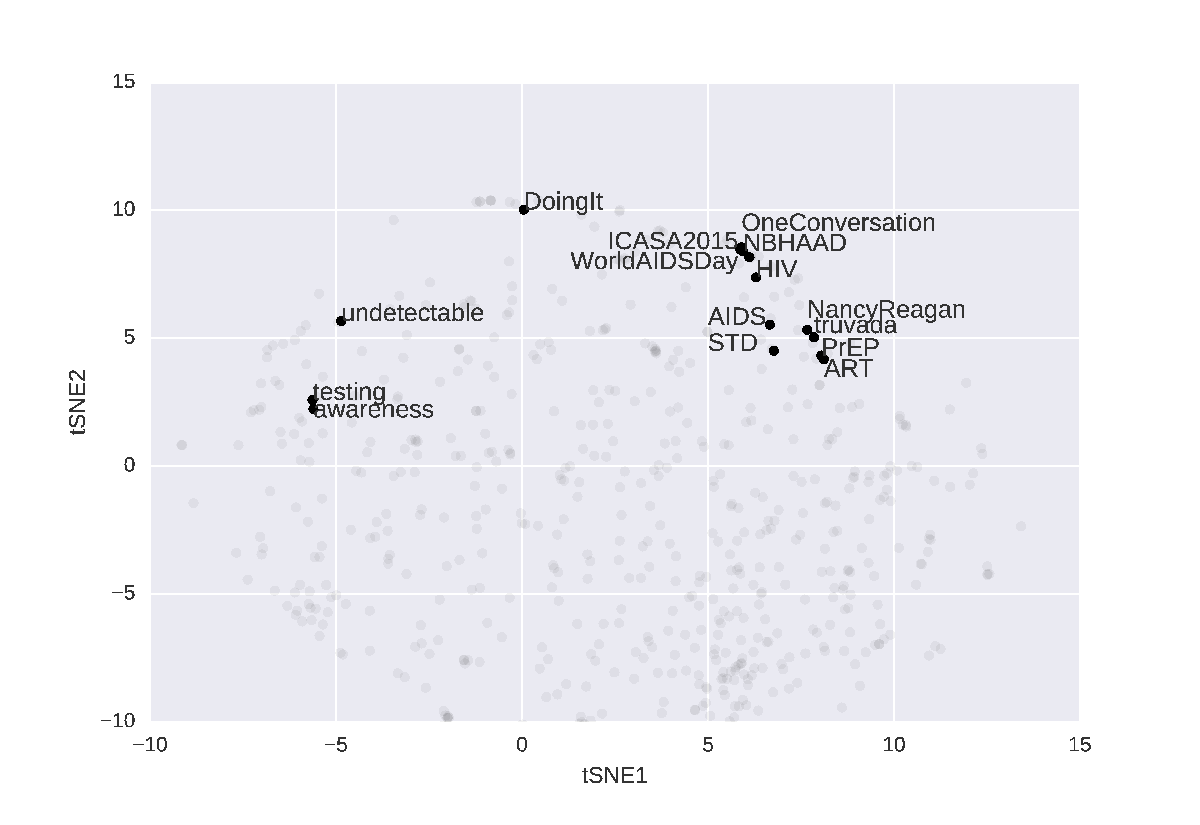
\includegraphics[height=4in, width=6in]{tSNE_word}
\caption{tSNE plot of relevant word-vectors}
\end{figure*}

\subsection{Time Domain}

Next we sought to identify some temporal trends in PrEP related trends. We used Dynamic Topic Modeling (DTM) to identify how certain topics change over time. We specified 10 topics and used each week's worth of tweets, over a 30 week period from the 47th week of 2015 to the 14th week of 2016, as our time points.

We identified two topics that showed relevant trends. In topic 5 we see that the keyword 'PrEP' increases over time, while 'prevention', 'drug' and 'risk' remain constant (Figure 3). The term 'pill', also from topic 5, declines overtime. These dynamics may indicate that PrEP discussion is becoming more prevalent. This growing trend would be consistent with the fact that while PrEP is still not widely known about among patients and healthcare providers, information about PrEP is slowly entering into national awareness. A study in New York City in 2011 indicated that only 36\% of high risk individuals were aware of PrEP~\cite{mehta2011awareness}.

Other HIV prevention related words such as 'pill', 'prevention' and 'drug' serve as negative controls. They are related to PrEP, but also used in other medical contexts. The fact that they are not increasing, shows us that the increase in PrEP discussion is PrEP-specific.

However, it is hard to tell from these data whether the increased level of PrEP discussion is leading to increased levels of informed patients, medical providers, and adherence. It is possible that stigma, and misinformation is leading to greater levels of PrEP discussion on twitter. We will get more specific, granular understanding of the PrEP discourse in our sentiment analysis section below (see section "Sentiment Classification").

% figure 3
\begin{figure}
\centering
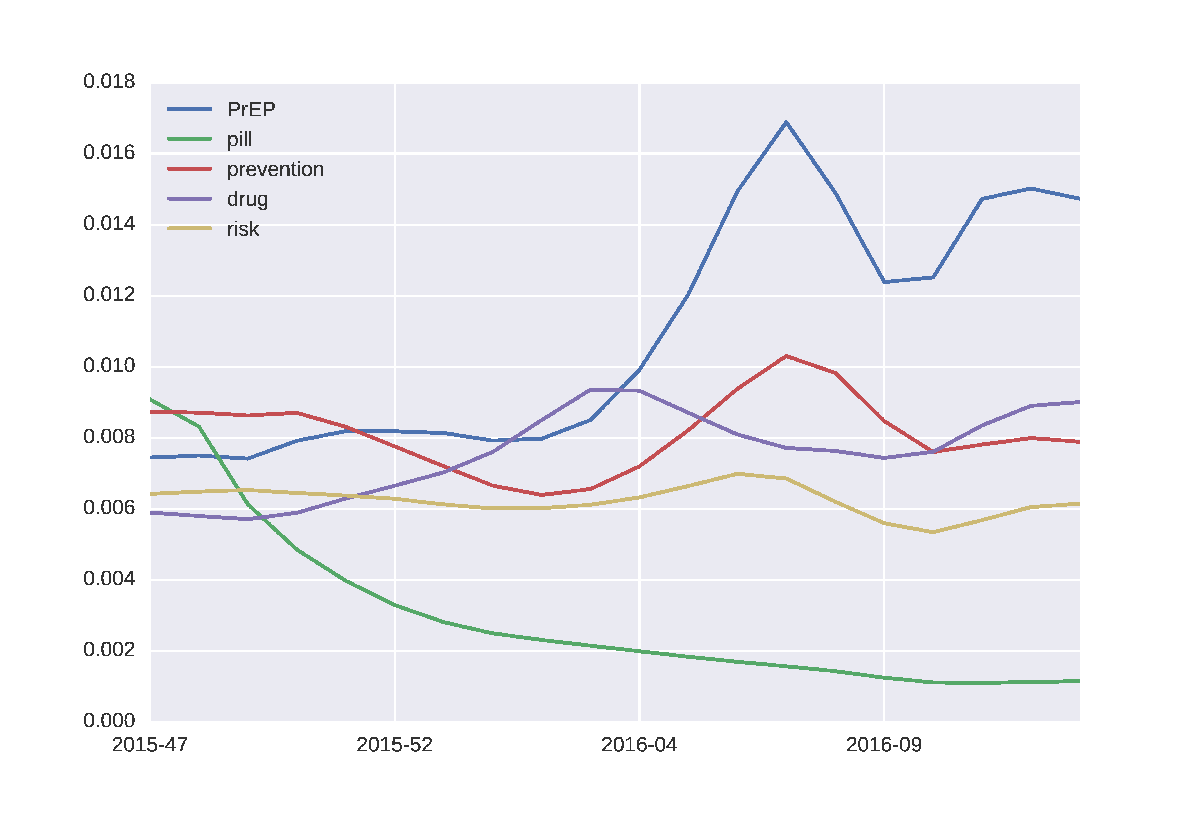
\includegraphics[height=2.5in, width=3.5in]{DTMfig1}
\caption{DTM topic 5 (PrEP related topic) word prevalence over time. Date is YYYY-WW.}
\end{figure}

We found at least one other DTM topic that showed interesting behavior. We observed that topic 4 captured several keywords related to World AIDS Day (Figure 4). We can see that "WorldAIDSDay", and "Can" peak in the 47th week of 2015 and then decline into 2016. This correlates well with the actual date of World AIDS Day, December 1st. Furthermore, while December 1st is World AIDS day, the whole month of December is AIDS Awareness Month. We can clearly see the words 'raise' and 'awareness' peak later and last longer than the word 'WorldAIDSDay' indicating that these words are correlated to the whole month of December. While our PrEP investigation isn't specifically interested in World AIDS Day, or AIDS Awareness Month, this observation serves as a control to validate our ability to accurately identify temporal events using DTM. 

% figure 4
\begin{figure}
\centering
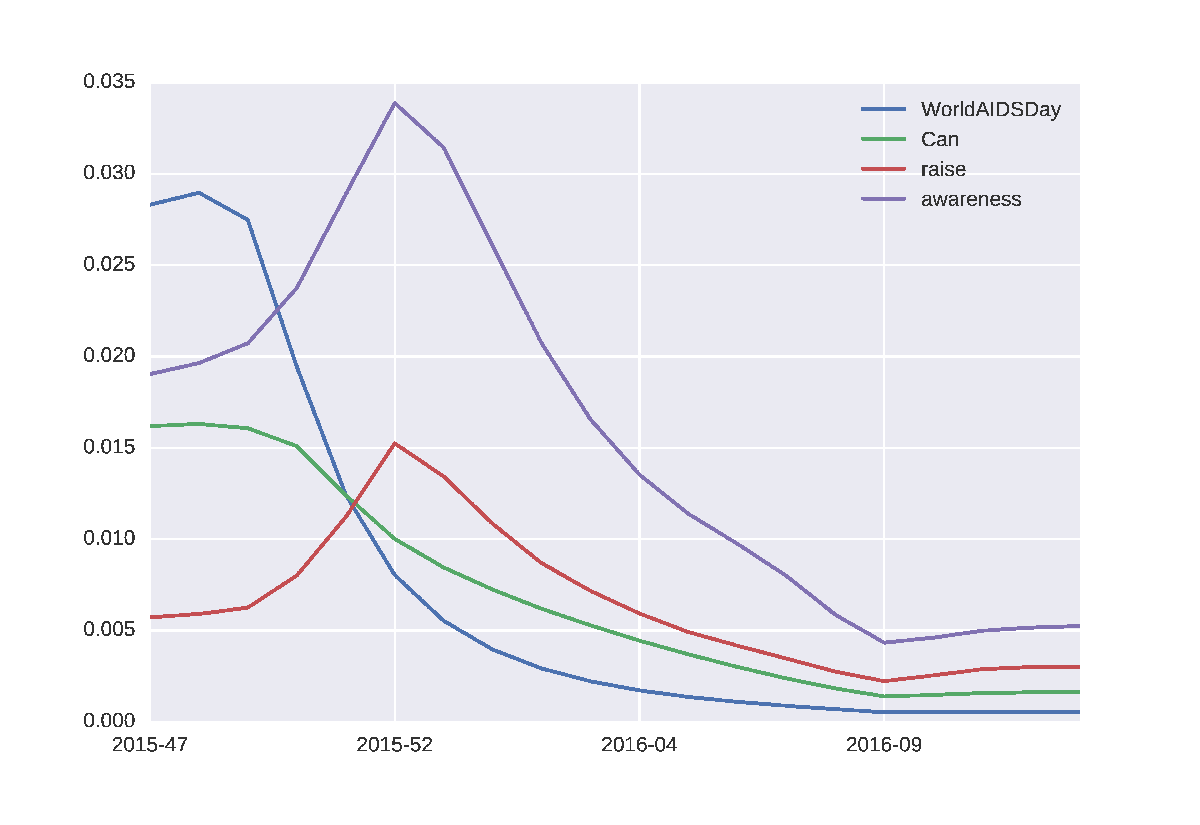
\includegraphics[height=2.5in, width=3.5in]{DTMfig2}
\caption{DTM topic 4 (WorldAIDSDay related topic) word prevalence over time. Date is YYYY-WW.}
\end{figure}

Together, the DTM results demonstrate our ability to extract relevant HIV and PrEP related information from Twitter that accurately captures time-dependent fluctuations. Public health professionals should be able to monitor these temporal trends to determine the relative interest in PrEP, and other HIV related keywords as they are discussed over time.

\subsection{User Timeline Analysis}

We wanted to identify what Twitter users that mentioned PrEP were discussing in their other tweets. We identified users that were most similar to PrEP using our Doc2Vec results, then downloaded their recent tweet history, up to their last 3000 tweets. We selected the top 500 users that had at least 200 total words in the combined tweets of their tweet history. For each user, we concatenated their timeline of tweets, and performed LDA topic modeling on the resulting set of user-timeline documents (Figure 5).

% figure 5
\begin{figure*}
\centering
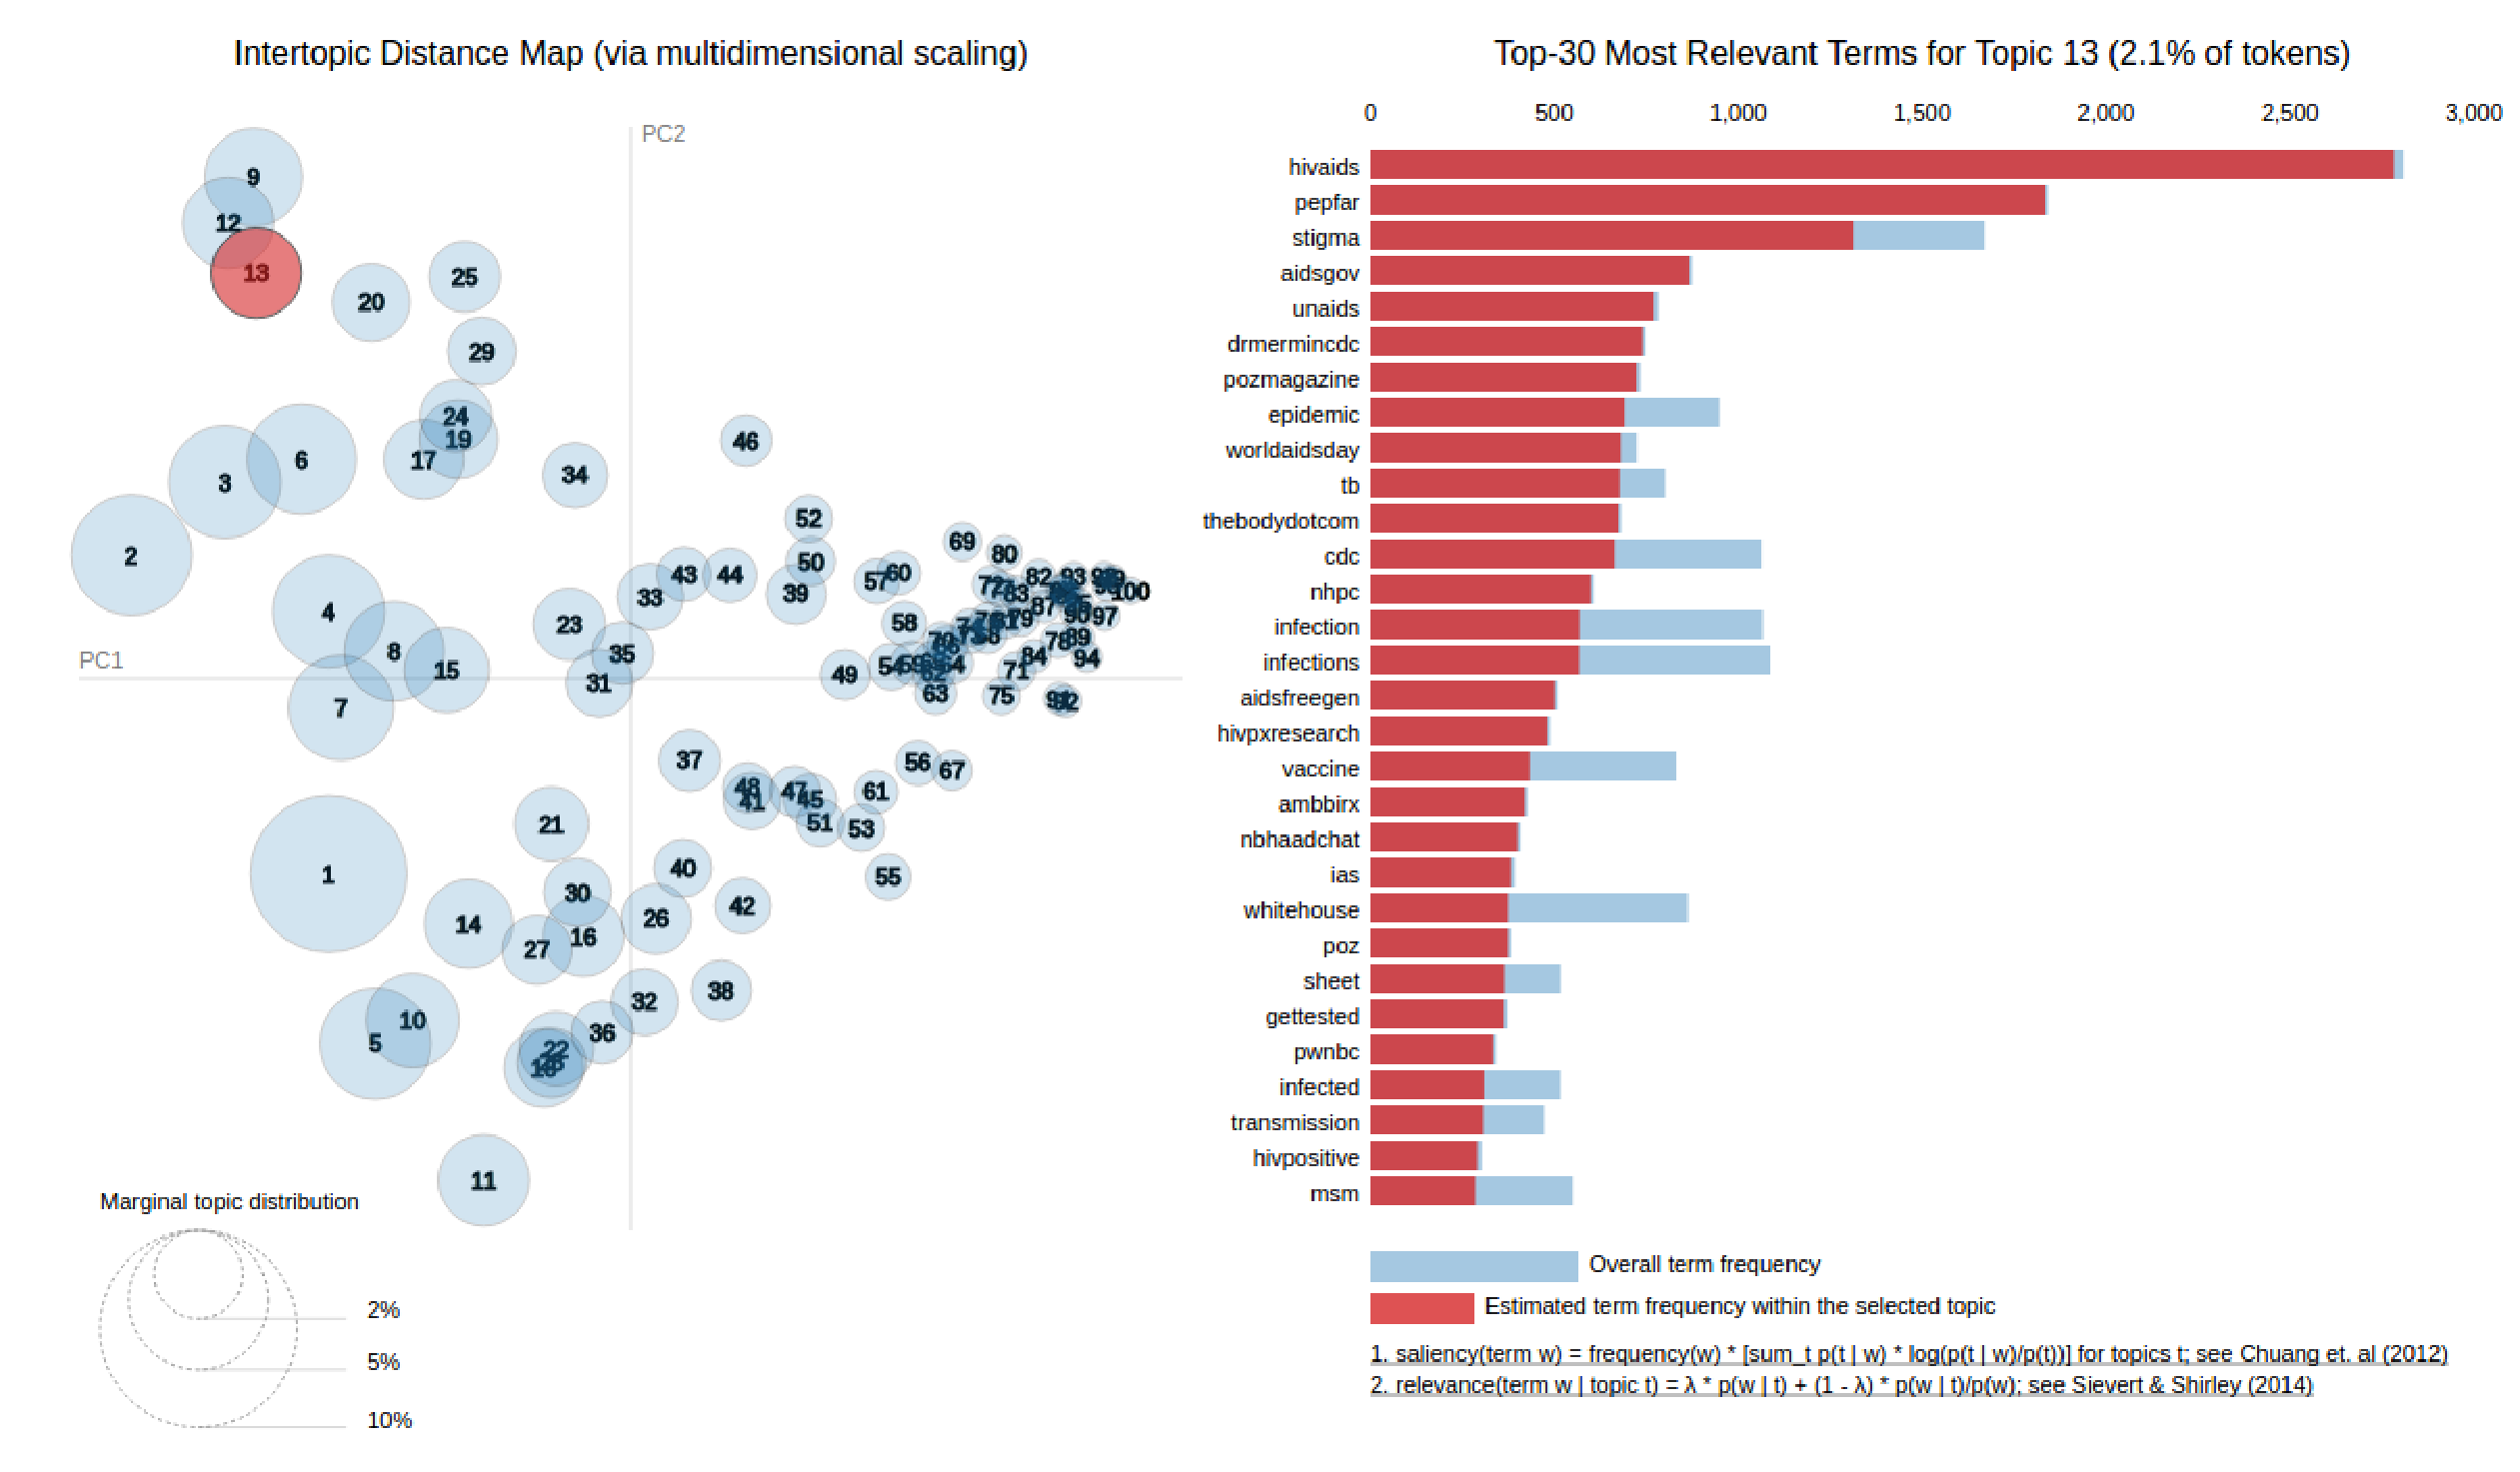
\includegraphics[height=2.5in, width=5in]{LDA_user_timelines}
\caption{Clustermap of users vs. topics for the top 500 users related to PrEP.}
\end{figure*}

We performed LDA on the users' timelines using the pyLDAvis python package from graphlab~\cite{low2014graphlab}. We specified 100 topics, and found that only one of them was related to HIV (topic number 13, see Figure 5) representing about 2\% of the marginal topic distribution. Topic 13 contained top terms "hivaids", "pepfar", "stigma" and "aidsgov". PEPFAR is a governmental organization, The United States President's Emergency Plan for AIDS Relief, that is focused on combating the spread of AIDS internationally. Interestingly, we don't see PrEP in the top 30 terms in topic 13. This indicates that among twitter users that talk about PrEP, HIV is a small part of their discussion, and PrEP an even smaller part of their discussion.

We investigated some of the other major topics from users' timelines, and found discussions of other STD's (topics 20, 29 and 17) and other health related terms (topics 12, and 25). The other health and STD-related topics clustered closely with topic 13 in Principle Component (PC) space. Some of the STD-related topics included terms related to LGBTQ, including the social networking platform Grindr in topic 17. Other terms related to STD's include prevention terms such as "CDC", "condoms", and "gettested". Topic 19 is nearby these STD-related topics in PC space, and contains terms related to healthcare and political issues such as "Obamacare" and "ACA" (Affordable Care Act). This connection between HIV, other STD prevention topics, and political discourse may be relevant in PrEP-based HIV prevention efforts, considering there is in some cases no clear precedent for how preventative therapies like PrEP are covered by health insurance~\cite{liu2014early}.

One of the top words from the HIV-related topic, topic 13, was the term "stigma", the term "endstigma" was also found in topic 17. Previous studies have shown a variety of stigmas associated and HIV have hampered prevention efforts~\cite{liu2014early}. Our observation of stigma related terms corroborates that there is some discussion of stigma in the context of HIV on Twitter. Public health professionals may be able use the prevalence of the term "stigma" as a way to monitor the efficacy of efforts to end HIV related stigmas.

\subsection{Sentiment Classification}

Previously, we used analyses to summarize the whole Twitter corpus to produce high level trends. For our final analysis, we sought to get a deeper understanding of the data at the individual tweet level. Thus we trained a classifier to classify the sentiment of HIV and PrEP related tweets to be either positive or negative. This classifier would allow public health professionals to quickly identify positive and negative PrEP related tweets to guide HIV prevention efforts. We obtained a set of 1.6 million tweets with binary sentiment labels from Sanders Analytics~\cite{sentimentdata}. Then we trained a simple logistic regression classifier on 1.2 million paragraph-vectors from the sentiment dataset. We found that our classifier had an accuracy of 69\% using a portion of the sentiment tweets not used in training, as a validation set.

We chose to use a relatively simple classifier model (logistic regression) and stop training at 20 epochs of stochastic gradient decent over the corpus, because we wanted to prevent the possibility that we overtrained on our training data. This was especially important because our training and testing data, while both sets of tweets, were separate datasets. We then used this trained classifier to classify our PrEP related tweets into positive or negative sentiment labels. We identified the most positive, and most negative tweets, by log probability, on our full dataset, and on tweets that specifically mention either PrEP or Truvada. We provide the text from the top three positive and negative tweets from each of the three datasets (Table 3, Table 4).

% do a top positive tweets table (also with tweet ID)
% table 3
\begin{table*}
\centering
\caption{Positive sentiment tweets.}
\begin{tabular}{|p{2.5cm}|p{12cm}|} \hline
Category & Text\\ \hline
General & "RT TOPublicHealth The Works provides testing for HIV anonymous \& rapid test available . Call 416-392-0520 for more info"\\ \hline
General & "RT FCAA ejaforg announced 5.4 million in grants to support orgs addressing \#HIV in new \& innovative ways!"\\ \hline
General & "RT HillaryClinton A note on the fight against HIV and AIDS and the people who really started the conversation."\\ \hline

PrEP specific & "He won't use condoms because intimacy means more than his health. but he's discovered PrEP. thank goodness."\\ \hline
PrEP specific & "PrEP Queensland Aids Council, \#HIV Foundation, Queensland."\\ \hline
PrEP specific & "RT JDatTheBody At the core of our programs is belief that young ppl can succeed in take PrEP for HIV prevention. \#NHPC2015"\\ \hline

Truvada specific & "RT CDC\_HIVAIDS Expanding testing, treatment, \& \#PrEP could prevent up to 185k new \#HIV infections"\\ \hline
Truvada specific & "Another reason 4 \#Ireland \& \#UK 2 immediately approve \#truvada \& \#PrEP 2 stop \#HIV infections . arleavitt AodhanORiordain MerchantsQuayIR"\\ \hline
Truvada specific & "RT EvanJPeterson For \#worldAIDSday my early \#PrEP arcticle in strangerslog, art by leviathanleague \#hiv \#truvada \#truvadawhore"\\ \hline

\hline\end{tabular}
\end{table*}

% do a top negative tweets table (also with tweet ID)
% table 4
\begin{table*}
\centering
\caption{Negative sentiment tweets.}
\begin{tabular}{|p{2.5cm}|p{12cm}|} \hline
Category & Text\\ \hline
General & "Also, how f***ing vile of Hillary to say. Reagan did f***ing NOTHING during the AIDS epidemic until it was too late. What a stupid old hag."\\ \hline
General & "I wonder why he beat her a** when she was tryna leave like she wasn't gone be running back when she found out she had HIV \& nobody want her"\\ \hline
General & "Aaannd. Hillary Clinton breathes a sigh of relief that Twitter has left its outrage of her AIDS comments behind to tend to Drumpf debacle."\\ \hline

PrEP specific & "RT gaston\_croupier \#Truvada patent's not expired yet but it is sold online as a generic drug? There's something rotten in internet \#PrEP h"\\ \hline
PrEP specific & "Equality\_MI Syph \& Hep C have gone up 550\% in Gay Men bc many feel tht bc they're on PrEP, they don't need condoms. HIV isn't the only STI."\\ \hline
PrEP specific & "Xaviom8 in interviews he says he was adherent. strain was highly resistant, and Truvada wouldn't have blocked it anyways. PrEP didn't fail."\\ \hline

Truvada specific & "not surprised at all that someone got HIV on truvada. people get pregnant on birth control. tomato-condoms are still important-tomahto"\\ \hline
Truvada specific & "Now reading that truvada does not protect against certain strains of the HIV virus. Yet people want to take that risk.."\\ \hline
Truvada specific & "I think I have conjunctivitis unless truvada cured it overnight cuz im not feeling as horrible today as last night"\\ \hline

\hline\end{tabular}
\end{table*}

While the sentiment classification doesn't have perfect sentiment accuracy, we can see in general that the positive tweets are disseminating information about the efficacy and benefits of PrEP related preventions (Table 3). The positive tweets indicate that PrEP public health informational efforts have had some effect disseminating PrEP information on Twitter. 

The negative tweets may be more important than the positive tweets to guide future public health policy corrections. The negative tweets contain concerns that Truvada may not block HIV transmission in all cases (Table 4). There also seems to be concern that use of Truvada may increase the transmission of non-HIV STDs such as Hepatitis C because some PrEP users stop using condoms. This may indicate that public health professionals need to stress that PrEP users should continue to wear condoms for full protection against other diseases when disseminating PrEP-related health information.

Another negative tweet questions whether Truvada is available as a generic drug. PrEP is currently only available through Gilead's Truvada, though a generic may be available as soon as 2017~\cite{truvadagenericblog}. Current patients must deal with uncertain drug prices, which vary from \$14,000 to \$70~\cite{truvadagenericblog}, and have in some cases, uncertain medical insurance reimbursement status. This tweet highlights both the difficulty of acquiring affordable PrEP medication, and also a level of conflicting information circulating on social media.

Finally we see some contention over national political leadership in the effort to prevent HIV. While political discussions can often get heated, especially on Twitter, the contention can harm concerted efforts to provide consent governmental leadership in HIV prevention. Public health officials may consider stressing that unity in health policy at the federal level is important to protect the population from the spread of HIV.

The last tweet in the positive tweets table (Table 3), referencing the hashtag "\#truvadawhore", links to a blog article written by Evan Peterson titled "The Case for PrEP, or How I Learned to Stop Worrying and Love HIV-Positive Guys"~\cite{caseforprep}. Evan is an HIV-negative individual who adheres to a daily PrEP regimen to protect himself from HIV. Evan finds that for himself, the side effects and inconveniences associated with taking daily Truvada are worth the protection, noting that he also practices safe sex, and gets tested regularly. Evan addresses the hashtag \#truvadawhore, which originated with a Huffington Post article titled "Truvada Whores?"~\cite{truvadawhore} which expressed concern toward the increased sexual risk taking of some Truvada patients. Evan notes that many HIV-negative individuals on Truvada like him who know that they may be exposed to HIV, are responsible and cautious about the risks they are taking. Individuals on Truvada may also be more informed than at risk people who do not use Truvada, because they are more educated and responsible with respect to their sexual health. Further large scale quantitative measurements will be needed to determine whether or not taking Truvada correlates with at risk behaviors.

\section{Conclusions}

In this article we use a variety of NLP techniques to analyze a tweet corpus in order to monitor the national social media discussion for HIV prevention. We identified several notable trends. Firstly, we found that PrEP discussion is increasing on social media, Secondly we found that people who mention PrEP also talk about general health, STDs, stigma, and politics.

By picking out the most relevant tweets to PrEP, and also classifying tweets as positive or negative, we quickly identified a handful of specific tweets that highlight important parts of the online PrEP discussion. We identified two important arguments for and against PrEP. One, as explored by blog author Steven Banning hypothesizes that PrEP adoption could lead to unintended, and unhealthy risk seeking behavior. The contrary hypothesis, described by blog author Evan Peterson, suggests that PrEP adoption is a product of healthy, responsible at-risk individuals who are gaining HIV protection in an effective form. These opposing arguments were identified automatically using large scale social media data. Further investigation and data analysis, of social media data, or other health data may be able to quantify PrEP and Truvada's effectiveness in the ongoing effort to prevent HIV infection.

Future analyses may also take advantage of the rich Twitter API. An additional refinement of the analyses presented here may take a more active approach. Rather than simple passive data collection, we could build a twitter bot to interact with HIV and PrEP-tweeters, or conduct a social media based health survey. Finally, future HIV and PrEP research may benefit from the incorporation of multiple data sources, either multiple social media sources, multiple health information sources, or both.

%\end{document}  % This is where a 'short' article might terminate

%ACKNOWLEDGMENTS are optional
\section{Acknowledgments}

Acknowledgements (optional) go here.

%
% The following two commands are all you need in the
% initial runs of your .tex file to
% produce the bibliography for the citations in your paper.

  % sigproc.bib is the name of the Bibliography in this case
% You must have a proper ".bib" file
%  and remember to run:
% latex bibtex latex latex
% to resolve all references
%
% ACM needs 'a single self-contained file'!
%
% no appendix for now...



\bibliographystyle{abbrv}
\bibliography{draft}



\end{document}
